\documentclass[MS]{wfuthesis}
\usepackage{graphicx} % Required for inserting images
\usepackage[utf8]{inputenc}
\usepackage{standalone}  % Allows including standalone .tex files
\usepackage{multicol}
\usepackage{amsmath, amssymb}
\usepackage{xcolor}
\usepackage{algorithm}
\usepackage{algpseudocode}
\usepackage{titlesec}
\usepackage[intoc]{nomencl} % To add abbreviations page, intoc adds it to the table of contents
\usepackage{etoolbox} % goes with the above package, to add groupings to the abbreviations
\usepackage[backend=biber, natbib=true, style=numeric, sorting=none]{biblatex}
\addbibresource{references.bib}

\titleformat{\chapter}[display]
  {\bfseries\Large}  % Format for the chapter title
  {}                 % No "Chapter X" label
  {0pt}              % Space between number and title
  {\Large}           % Additional formatting for the title


\title{\textbf{Advances in Tensor Decompositions: Fast Matrix Multiplication Algorithms And Parallel Adaptive Compression Techniques}}
\author{\textbf{João Victor de Oliveira Pinheiro}}
\date{May 2025}
\linespread{1.5}

\department{Computer Science}
\advisor{Grey Ballard, Ph.D.}
\chairperson{Aditya Devarakonda, Ph.D.}
\member{Frank Moore, Ph.D.}
\member{Ramakrishnan Kannan, Ph.D.}






%%%%%%%%%%%%%%%%%%%%%%%%%
%% My Own Shennenigans %%
%%%%%%%%%%%%%%%%%%%%%%%%%

\definecolor{mycustomgreen}{RGB}{44, 183, 66}
\definecolor{mycustomorange}{RGB}{255, 149, 1}
\definecolor{mycustompurple}{RGB}{181, 29, 227}

\makenomenclature
\renewcommand{\nomname}{\textbf{LIST OF ABREVIATIONS}}
\renewcommand\nomgroup[1]{%
  \item[\bfseries
  \ifstrequal{#1}{P}{Physics constants}{%
  \ifstrequal{#1}{N}{Number sets}{%
  \ifstrequal{#1}{O}{Other symbols}{}}}%
]}




%%%%%%%%%%%%
%% THESIS %%
%%%%%%%%%%%%

\begin{document}
    \maketitle
    %%%%%%%%%%%%%%%%%%%%%%
    %% Acknowledgements %%
    %%%%%%%%%%%%%%%%%%%%%%
    \section*{\textbf{ACKNOWLEDGEMENTS}} To all of those that came before me, and to all of those who are yet to come





    %%%%%%%%%%%%%%%%%%%%%%%
    %% Table of Contents %%
    %%%%%%%%%%%%%%%%%%%%%%%
    \tableofcontents
    \newpage




    %%%%%%%%%%%%%%%%%%%%%%%%%%%
    %% List of Illustrations %%
    %%%%%%%%%%%%%%%%%%%%%%%%%%%
    % \addcontentsline{toc}{chapter}{\textbf{LIST OF ILLUSTRATIONS}}
    % \begin{center}
    %     \textbf{LIST OF ILLUSTRATIONS}
    % \end{center}
    \listoffigures
    \newpage




    %%%%%%%%%%%%%%%%%%%%%%%%%%
    %% List of Abreviations %%
    %%%%%%%%%%%%%%%%%%%%%%%%%%
    % \addcontentsline{toc}{chapter}{\textbf{LIST OF ABREVIATIONS}}
    % \begin{center}
    %     \textbf{LIST OF ABREVIATIONS}
    % \end{center}
    \nomenclature[P]{\(c\)}{Speed of light in a vacuum}
    \nomenclature[P]{\(h\)}{Planck constant}
    \nomenclature[P]{\(G\)}{Gravitational constant}
    \nomenclature[N]{\(\mathbb{R}\)}{Real numbers}
    \nomenclature[N]{\(\mathbb{C}\)}{Complex numbers}
    \nomenclature[N]{\(\mathbb{H}\)}{Quaternions}
    \nomenclature[O]{\(V\)}{Constant volume}
    \nomenclature[O]{\(\rho\)}{Friction index}

    \printnomenclature
    \newpage






    %%%%%%%%%%%%%%
    %% Abstract %%
    %%%%%%%%%%%%%%
    \addcontentsline{toc}{chapter}{\textbf{ABSTRACT}}
    \begin{center}
        \textbf{ABSTRACT}
    \end{center}
    This thesis is built on two projects. They all fall under Tensor
    Decompositions as the title states. Here I present the abstracts for the two
    projects separately, in chronological order in which I began working on
    them.

    \textbf{Searching For Fast Matrix Multiply Algorithms using Cyclic-Invariant
    CP decomposition:} Fast matrix multiplication algorithms correspond to exact
    CP decompositions of tensors that encode matrix multiplication of fixed
    dimensions. This 3-way matrix multiplication tensor M has cyclic symmetry:
    the entry values are invariant under cyclic permutation of the indices. The
    CP decomposition of Strassen’s original fast matrix multiplication algorithm
    for 2x2 matrices is cyclic invariant, and cyclic invariant decompositions
    are known to exist for 3x3 and 4x4 matrix multiplication as well. Cyclic
    invariance means a cyclic permutation of the CP factors results in the same
    CP components, just in a different order. We describe how to search for
    these solutions, which involve one third of the variables of generic
    solutions, using the damped Gauss-Newton optimization method along with
    heuristic rounding techniques, and we summarize the algorithms discovered so
    far.

    \textbf{Parallel Higher-Order Orthogonal Iteration for Tucker Decomposition
    with Rank Adaptivity:} Higher Order Orthogonal Iteration (HOOI) is an
    algorithm that uses block coordinate descent optimization to compress an
    input tensor into a Tucker format approximation. Classical HOOI requires
    specifying the ranks, or dimensions of the core tensor, and seeks to
    minimize the approximation error. 	We introduce HOOI-Adapt, a novel
    error-specified algorithm that adaptively selects the ranks of the Tucker
    tensor in order to maximize the compression subject to the error threshold.
    We implement HOOI-Adapt using the distributed-memory parallel TuckerMPI
    library and employ memoization to reduce the computational cost.
    Furthermore, we show that when the ranks are small, HOOI-Adapt has lower
    computational cost compared to the alternative Sequentially Truncated
    Higher-Order SVD (ST-HOSVD) algorithm. Our benchmarks demonstrate that our
    parallel implementation of HOOI-Adapt outperforms TuckerMPI’s ST-HOSVD for
    small ranks when scaled to terabyte-sized input datasets on NERSC’s
    Perlmutter platform.





    %%%%%%%%%%%%%%%%%%
    %% Introduction %%
    %%%%%%%%%%%%%%%%%%
    \chapters{}
    \chapter{\textbf{Introduction}}

        %%%%%%%%%%%%%%%%%%%%%%%
        %% Problem Statement %%
        %%%%%%%%%%%%%%%%%%%%%%%
        \section{What Is A Tensor?}
            There is no widely agreed definition of a tensor; different fields
            define it differently. In March 2024, Mathematics Professor Thomas
            Lam at NYU conducted an online informal survey on mathematical
            conventions \cite{Math_Conventions_Survey}. The title of this first
            section is named after question 45 of that survey, \textit{What is a
            Tensor?}. Its results can be seen on Figure \ref{fig:What Is A
            Tensor?}. Though the target audience for this survey were mostly
            mathematicians and mathematics enthusiats, we can still observe a
            lerge variaty in definitions of a tensor. But in the great words of
            my advisor \textit{``94\% of people are wrong''}, and so we reach the
            definition: \textbf{a tensor is a multidimensional array}.
            
            In other words, a tensor is a $d$-way array, where $d$ is referred
            to as the order of the tensor.

            \begin{figure}
                \centering
                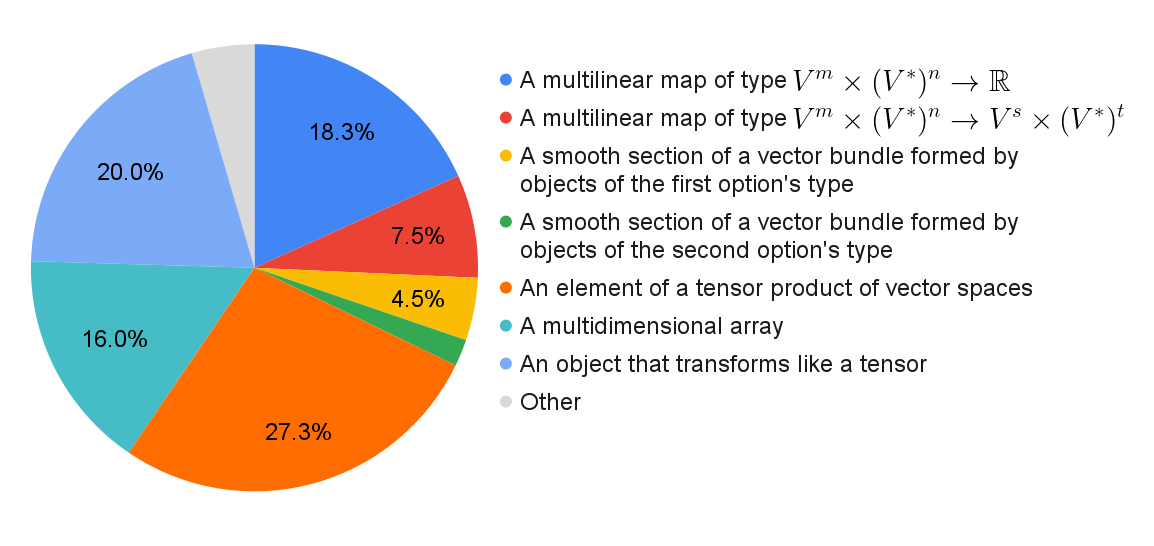
\includegraphics[width=\textwidth]{Figures/WhatIsATensor.png}
                \caption[Figure \ref{fig:What Is A Tensor?} - What Is A Tensor?]{What Is A Tensor?}
                \label{fig:What Is A Tensor?}
            \end{figure}

        \section{Problem Statement} % The importance of the problem
            \subsection{Preliminaries}
                A tensor is a multidimensional array. Think of an array as an 1D tensor, a matrix as a 2D tensor, a 3D tensor is a cube of data, a 4D tensor is an array of 3D tensors, a 5D a matrix of 3D tensors, and it generalizes onwards. Similarly, a scalar can be thought of as a 0D tensor. The number of entries stored in memory is the product of each dimension size. A 1D tensor (an array) has $n$ entries, a 2D Tensor (a matrix) has $n^2$ entries, a 3D tensor has $n^3$ and so on. As you can imagine, the memory footprint of a tensor gets larger and larger the more dimensions and the bigger their sizes are. Because they get memory expensive so quickly, there are ways to compress these multidimensional arrays that go beyond the regular zipping of a file. \textit{consider motivating why we prefer this over regular file compression.} We call the compression of a tensor to be a \textbf{tensor decomposition} because it relies on decomposing the full tensor into smaller subpart that when multiplied together we get an approximation of the original tensor. Though there are only a couple of types of tensor decompositions, each type of decomposition has many algorithms of which we will only focus on a few on this thesis. We will only cover two types of tensor decompositions, one belonging to each project:
                
                \subsubsection{Tucker Tensor}
                    This is the type of tensor used on project 2. A Tucker Tensor (TTensor) is a core tensor with as many factor matrices as there are dimensions which are multiplied with the core to reconstruct the global tensor as in Figure \ref{fig:TTensor_the}.
                    
                    \begin{figure}[ht]
                        \centering
                        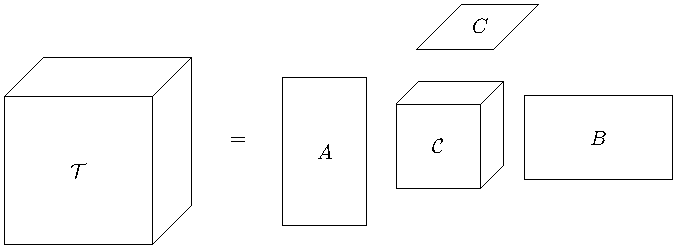
\includegraphics[scale=1]{tikz/Tucker_Tensor.pdf}
                        \caption{A 3 way Tucker Tensor Diagram}
                        \label{fig:TTensor_the}
                    \end{figure}

                    If we consider a 3D tensor of size $n^3$ with core of size $r^3$ where $r < n$. Then the number of entries of a TTensor is $3rn + r^3$ which is less than the original memory footprint and much less if $r \ll n$. The approximation gets more accurate with a bigger core tensor, which implies a trade-off between compression and accuracy. The traditional methods are HOSVD (Higher Order Singular Value Decomposition) and STHOSVD (Sequentially Truncated Singular Value Decomposition). HOOI (Higher Order Orthogonal Iteration) was the last to be added to this list, this is the method project 2 builds on. STHOSVD and HOOI can be seen in Algorithms \ref{alg:STHOSVD} and \ref{alg:Classic-HOOI}.
                    
                
                \subsubsection{Kruskal Tensor}
                    This tensor decomposition format is used on project 1. A Kruskal Tensor (KTensor) is a number of $d$ outer products of vectors of length $n$, the number of outer products is the rank of the KTensor namely $R$, which can be seen in Figure \ref{fig:KTensor}.
                    \begin{figure}[ht]
                        \centering
                        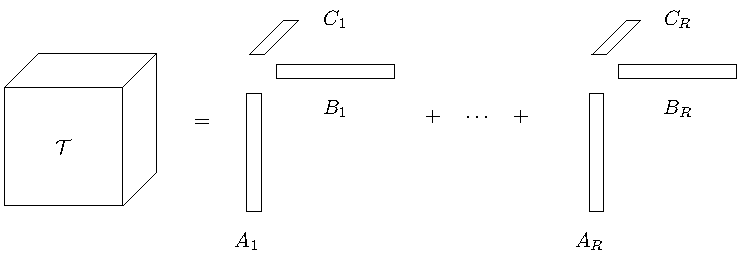
\includegraphics[scale=1]{tikz/CP_Tensor.pdf}
                        \caption{A 3 way CP Tensor Diagram}
                        \label{fig:KTensor}
                    \end{figure}
                    The memory footprint of a K Tensor is $3Rn$. The approximation gets more accurate as $R$ increases. This is the 2D the matrix equivalent of having a matrix approximation to be the outer product of two vectors as an $n \times 1$ array times a $1 \times n$ array equals an $n \times n$ matrix. The traditional methods are gradient descent and the newton method. The process of compressing a d-way tensor into a K Tensor is called a CP Decomposition, there are several CP Decomposition methods, but we focus on the damped gauss newton (CP-DGN) optimization method which can be found in Algorithm \ref{alg:CP-DGN}.

                \subsubsection{Tensor Train}
                    This tensor decomposition format is used on project 3. A Tensor Train Tensor (TT Tensor) takes a $d$-way tensor and compresses it into a product of two outer matrices and $d-2$ 3way cores.
                    \begin{figure}[ht]
                        \centering
                        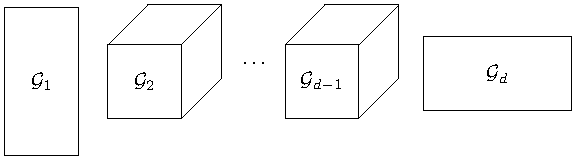
\includegraphics[scale=1]{tikz/Tensor_Train.pdf}
                        \caption{A $d$ way Tensor Train Diagram}
                    \end{figure}
                    The memory footprint of a TT tensor is $2nr + dnr^2$, and it is quite effective for tensor with multiple dimensions. The traditional method for TT is the TT-SVD.

                \subsection{The Matrix Multiplication Tensor}
                    There is a specific type of tensor that will be necessary for the understanding of the first project; the Matrix Multiplication Tensor. We assume the reader is already familiar with matrix matrix multiplication, which makes its tensor format easier to comprehend. It is a 3D tensor which holds the matrix multiplication algorithm. We can create this tensor for any two matrices $m\times n$ times an $n \times p$. The dimension of the matrix multiplication tensor would then be $m^2 \times n^2 \times p^2$. To successfully multiply two matrices using the tensor, we vectorize the two matrices and multiply against the first and second dimensions of the tensor, respectively, to get the output you normally get in matrix multiplication, as shown on Figure \ref{fig:MatMulTensor}.
                    \begin{figure}[ht]
                        \centering
                        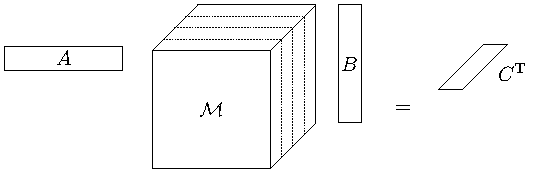
\includegraphics[scale=1]{tikz/MatMul_asTensor.pdf}
                        \caption{Matrix Multiplication in Tensor Format}
                        \label{fig:MatMulTensor}
                    \end{figure}

                

            \subsection{The Importance of Tensor Decompositions}
                \subsubsection{Tensor Decompositions for Data Compression ($2^\text{nd} \text{ and } 3^\text{rd}$ projects)}
                    As discussed earlier, the memory footprint increases quickly as the number of dimensions increases as well as its sizes. Since the size of a tensor is its dimensions multiplied, an increased in just a single of its dimensions can result in an extremely larger tensor. In fact the TT tensor is an effective option for tensors with many dimensions as the storage is exponential in the number of dimensions (recall storage cost is $n^d$ for a uniform tensor). This happens because the Tucker Tensor still has exponential in $d$ storage $r^d$ which the TT tensor does not.
                    
                    Because of the high cost of storing raw tensors, tensor decompositions are highly effective in reducing tensor storage. However, we cannot decrease memory footprints without first losing some accuracy. Classic HOOI, STHOSVD, and the TTSVD algorithms allow the user to specify the dimensions of the core tensor. Often times just specifying the dimensions does not mean the user will know how much error it will introduce to the tensor. This is not a problem for STHOSVD and TTSVD since those have an error-specified variant that the HOOI algorithm does not.

                \subsubsection{Tensor Decompositions for Interpretations ($1^\text{st}$ project)}
                    Recall that matrix multiplication is an $O(n^3)$ algorithm. But we can decrease this cost by using Strassen's Algorithm as shown below:

                    \begin{multicols}{2}
                        \textbf{Classic Algorithm}
                            \begin{eqnarray*}
                                \color{blue} M_1 & = & A_{11}\cdot B_{11} \\
                                \color{blue} M_2 & = & A_{12}\cdot B_{21} \\
                                \color{blue} M_3 & = & A_{11}\cdot B_{12} \\
                                \color{blue} M_4 & = & A_{12}\cdot B_{22} \\
                                \color{blue} M_5 & = & A_{21}\cdot B_{11} \\
                                \color{blue} M_6 & = & A_{22}\cdot B_{21} \\
                                \color{blue} M_7 & = & A_{21}\cdot B_{12} \\
                                \color{blue} M_8 & = & A_{22}\cdot B_{22} \\
                                C_{11} & = & \color{blue} M_1 \color{black} + \color{blue} M_2 \\
                                C_{12} & = & \color{blue} M_3 \color{black} + \color{blue} M_4 \\
                                C_{21} & = & \color{blue} M_5 \color{black} + \color{blue} M_6 \\
                                C_{22} & = & \color{blue} M_7 \color{black} + \color{blue} M_8
                            \end{eqnarray*}
                            \vspace{-40pt}
                            \begin{eqnarray*}
                                \text{8 multiplies, 4 additions} \\
                                T(n) = 8T(n/2) + O(n^2) \\
                                T(n) = O(n^{log_2 8}) = O(n^3)
                            \end{eqnarray*}
                            
                        \columnbreak

                        \textbf{Strassen's Algorithm}
                            \begin{eqnarray*}
                                \color{blue} M_1 & = & (A_{11} + A_{22})\cdot (B_{11} + B_{22}) \\
                                \color{blue} M_2 & = & (A_{12} + A_{22})\cdot B_{11} \\
                                \color{blue} M_3 & = & A_{11}\cdot (B_{21} - B_{22}) \\
                                \color{blue} M_4 & = & A_{22}\cdot (B_{12} - B_{11}) \\
                                \color{blue} M_5 & = & (A_{11} + A_{21})\cdot B_{22} \\
                                \color{blue} M_6 & = & (A_{12} - A_{11})\cdot (B_{11} + B_{21}) \\
                                \color{blue} M_7 & = & (A_{21} - A_{22})\cdot (B_{12} + B_{22}) \\
                                C_{11} & = & \color{blue} M_1 \color{black} + \color{blue} M_4 \color{black} - \color{blue} M_5 \color{black} + \color{blue} M_7 \\
                                C_{12} & = & \color{blue} M_3 \color{black} + \color{blue} M_5 \\
                                C_{21} & = & \color{blue} M_2 \color{black} + \color{blue} M_4 \\
                                C_{22} & = & \color{blue} M_1 \color{black} - \color{blue} M_2 \color{black} + \color{blue} M_3 \color{black} + \color{blue} M_6
                            \end{eqnarray*}
                            \vspace{-40pt}
                            \begin{eqnarray*}
                                \text{7 multiplies, 18 additions} \\
                                T(n) = 7T(n/2) + O(n^2) \\
                                T(n) = O(n^{log_2 7}) = O(n^{2.81})
                            \end{eqnarray*}
                    \end{multicols}

                    This is a product of the recursive implementation of Strassen's algorithm, the less recursive calls we do, the less expensive our algorithm will be as shown by the cost analysis above. For the $2 \times 2$ case we know we cannot improve the 7 multiplies from \textit{insert reference here}. Furthermore, we also know that Strassen's algorithm is not unique. We can rearrange the additions and multiplies to get another algorithm with the same number of multiplies and additions. We could search for different solutions that all have the same cost by performing an optimization search on each parameter involved in matrix multiplication as seen in Figure \ref{Opt}:

                    \begin{figure}
                        \centering
                        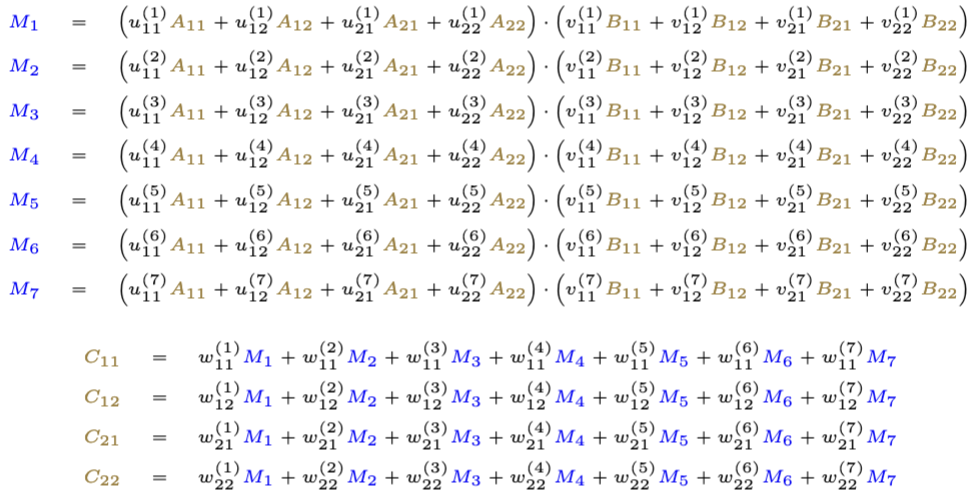
\includegraphics[scale=0.75]{Figures/MatMulAlgSearch.png}
                        \caption{The optimization search for Matrix Multiply Algorithms for the $2 \times 2$ case involving 7 multiplications. The number of variables is $4 \cdot 7 \cdot 3 = 84$. If we are searching for a discrete solution with only $-1, 0, 1$ as coefficients then we have $3^{84} \approx 10^{40}$ possibilities}
                        \label{Opt}
                    \end{figure}

                    \newpage

                    Below is one of these Strassen's variant algorithm next to the original. Strassen's algorithm has an underlying structure that this project relies on. However, it is not visible on the original layout. Strassen's algorithm is \textbf{Cyclic Invariant}. This is hard to visualize with only this presentation. Instead, we must turn to tensors to understand this structure.

                    \newpage
                    \begin{multicols}{2}
                        \textbf{Strassen's Algorithm}
                            \begin{eqnarray*}
                                \color{blue} M_1 & = & (A_{11} + A_{22})\cdot (B_{11} + B_{22}) \\
                                \color{blue} M_2 & = & (A_{12} + A_{22})\cdot B_{11} \\
                                \color{blue} M_3 & = & A_{11}\cdot (B_{21} - B_{22}) \\
                                \color{blue} M_4 & = & A_{22}\cdot (B_{12} - B_{11}) \\
                                \color{blue} M_5 & = & (A_{11} + A_{21})\cdot B_{22} \\
                                \color{blue} M_6 & = & (A_{12} - A_{11})\cdot (B_{11} + B_{21}) \\
                                \color{blue} M_7 & = & (A_{21} - A_{22})\cdot (B_{12} + B_{22}) \\
                                C_{11} & = & \color{blue} M_1 \color{black} + \color{blue} M_4 \color{black} - \color{blue} M_5 \color{black} + \color{blue} M_7 \\
                                C_{12} & = & \color{blue} M_3 \color{black} + \color{blue} M_5 \\
                                C_{21} & = & \color{blue} M_2 \color{black} + \color{blue} M_4 \\
                                C_{22} & = & \color{blue} M_1 \color{black} - \color{blue} M_2 \color{black} + \color{blue} M_3 \color{black} + \color{blue} M_6
                            \end{eqnarray*}
                            
                        \columnbreak

                        \textbf{Variant of Strassen's Algorithm}
                            \begin{eqnarray*}
                                \color{blue} M_1 & = & (A_{11} + A_{22})\cdot (B_{11} + B_{22}) \\
                                \color{blue} M_2 & = & (A_{12} + A_{22})\cdot B_{11} \\
                                \color{blue} M_3 & = & A_{22}\cdot (B_{12} - B_{11}) \\
                                \color{blue} M_4 & = & (A_{21} - A_{22})\cdot (B_{12} + B_{22}) \\
                                \color{blue} M_5 & = & (A_{11} + A_{21})\cdot B_{22} \\
                                \color{blue} M_6 & = & A_{11}\cdot (B_{21} - B_{22}) \\
                                \color{blue} M_7 & = & (A_{12} - A_{11})\cdot (B_{11} + B_{21}) \\
                                C_{11} & = & \color{blue} M_1 \color{black} + \color{blue} M_3 \color{black} - \color{blue} M_4 \color{black} - \color{blue} M_6 \\
                                C_{12} & = & \color{blue} M_2 \color{black} + \color{blue} M_3 \\
                                C_{21} & = & \color{blue} M_5 \color{black} + \color{blue} M_6 \\
                                C_{22} & = & \color{blue} M_1 \color{black} - \color{blue} M_2 \color{black} + \color{blue} M_5 \color{black} + \color{blue} M_7
                            \end{eqnarray*}
                    \end{multicols}

                    Recall that for a CP-Tensor, its rank is the number of components, but they can also be viewed as the number of columns of the factor matrices. When we decompose the matrix multiplication tensor we can find matrix multiplications algorithms embedded into its CP decomposition! Furthermore, the rank of the CP decomposition corresponds to the number of multiplications in the algorithm. Therefore, we can actively search for matrix multiplication algorithms with specified number of multiplications by decomposing the MatMul tensor. The CP decomposition that contains both Strassen's Algorithm and its variant is shown below. The three blocks represent the three factor matrices, and the columns are the components of the `chicken feet' in Figure 3.
        `           
                    \newpage
                    \begin{multicols}{2}
                        \[\begin{array}{c|ccccccc}
                                & M_1 & M_2 & M_3 & M_4 & M_5 & M_6 & M_7 \\
                                \hline
                                A_{11} & 1 & 0 & 1 & 0 & 1 & -1 & 0 \\
                                A_{12} & 0 & 1 & 0 & 0 & 0 & 1 & 0 \\
                                A_{21} & 0 & 0 & 0 & 0 & 1 & 0 & 1 \\
                                A_{22} & 1 & 1 & 0 & 1 & 0 & 0 & -1 \\
                                \hline
                                B_{11} & 1 & 1 & 0 & -1 & 0 & 1 & 0 \\
                                B_{12} & 0 & 0 & 0 & 1 & 0 & 0 & 1 \\
                                B_{21} & 0 & 0 & 1 & 0 & 0 & 1 & 0 \\
                                B_{22} & 1 & 0 & -1 & 0 & 1 & 0 & 1 \\
                                \hline
                                C_{11} & 1 & 0 & 0 & 1 & -1 & 0 & 1 \\
                                C_{21} & 0 & 0 & 1 & 0 & 1 & 0 & 0 \\
                                C_{12} & 0 & 1 & 0 & 1 & 0 & 0 & 0 \\
                                C_{22} & 1 & -1 & 1 & 0 & 0 & 1 & 0 \\
                        \end{array}\]
                    
                        \columnbreak
                        
                        \[\begin{array}{c|ccccccc}
                                & M_1 & M_2 & M_3 & M_4 & M_5 & M_6 & M_7 \\
                                \hline
                                A_{11} & \color{red} 1 & \color{mycustomgreen} 0 & \color{mycustomgreen} 0 & \color{violet} 0 & \color{violet} 1 & \color{orange} 1 & \color{orange} -1 \\
                                A_{12} & \color{red} 0 & \color{mycustomgreen} 1 & \color{mycustomgreen} 0 & \color{violet} 0 & \color{violet} 0 & \color{orange} 0 & \color{orange} 1 \\
                                A_{21} & \color{red} 0 & \color{mycustomgreen} 0 & \color{mycustomgreen} 0 & \color{violet} 1 & \color{violet} 1 & \color{orange} 0 & \color{orange} 0 \\
                                A_{22} & \color{red} 1 & \color{mycustomgreen} 1 & \color{mycustomgreen} 1 & \color{violet} -1 & \color{violet} 0 & \color{orange} 0 & \color{orange} 0 \\
                                \hline
                                B_{11} & \color{red} 1 & \color{orange} 1 & \color{orange} -1 & \color{mycustomgreen} 0 & \color{mycustomgreen} 0 & \color{violet} 0 & \color{violet} 1 \\
                                B_{12} & \color{red} 0 & \color{orange} 0 & \color{orange} 1 & \color{mycustomgreen} 1 & \color{mycustomgreen} 0 & \color{violet} 0 & \color{violet} 0 \\
                                B_{21} & \color{red} 0 & \color{orange} 0 & \color{orange} 0 & \color{mycustomgreen} 0 & \color{mycustomgreen} 0 & \color{violet} 1 & \color{violet} 1 \\
                                B_{22} & \color{red} 1 & \color{orange} 0 & \color{orange} 0 & \color{mycustomgreen} 1 & \color{mycustomgreen} 1 & \color{violet} -1 & \color{violet} 0 \\
                                \hline
                                C_{11} & \color{red} 1 & \color{violet} 0 & \color{violet} 1 & \color{orange} 1 & \color{orange} -1 & \color{mycustomgreen} 0 & \color{mycustomgreen} 0 \\
                                C_{21} & \color{red} 0 & \color{violet} 0 & \color{violet} 0 & \color{orange} 0 & \color{orange} 1 & \color{mycustomgreen} 1 & \color{mycustomgreen} 0 \\
                                C_{12} & \color{red} 0 & \color{violet} 1 & \color{violet} 1 & \color{orange} 0 & \color{orange} 0 & \color{mycustomgreen} 0 & \color{mycustomgreen} 0 \\
                                C_{22} & \color{red} 1 & \color{violet} -1 & \color{violet} 0 & \color{orange} 0 & \color{orange} 0 & \color{mycustomgreen} 1 & \color{mycustomgreen} 1 \\
                        \end{array}\]
                        
                    \end{multicols}
                    
                    By simply rearranging the columns of the original algorithm, the cyclic structure the algorithm can be seen in the colors of the decomposition. Notice how we have repeats of the same subcomponents in a cyclic form, they are called the \textbf{cyclic components} of the decomposition. That is we have green-purple-orange, then orange-green-purple and lastly purple-orange-green. The red color up front does not cycle, but is repeated in all three factor matrices, that is called the \textbf{symmetric component}. It is called that way because if we reshape that vector into a $2 \times 2$ matrix, it becomes a symmetric matrix. We can reduce the number of variables we must search from the $3^{84}$ possibilities to just $3^{28}$ possibilities. This however does not mean that exhausting the cyclic invariant solutions implies exhausting all solutions. As the original Strassen algorithm shows us, not all solutions are cyclic invariant. Now we can change the number of columns that are symmetric which would then change the number of columns that are cyclic. As long as we have that number of columns is equal to the number of columns in the symmetric component plus 3 times the number of columns in the cyclic component. In other words: \(R = Rs + 3Rc\):

                    \begin{multicols}{2}
                        \[\begin{array}{c|ccccccc}
                                & M_1 & M_2 & M_3 & M_4 & M_5 & M_6 & M_7 \\
                                \hline
                                A_{11} & \color{red} 1 & \color{mycustomgreen} 0 & \color{mycustomgreen} 0 & \color{violet} 0 & \color{violet} 1 & \color{orange} 1 & \color{orange} -1 \\
                                A_{12} & \color{red} 0 & \color{mycustomgreen} 1 & \color{mycustomgreen} 0 & \color{violet} 0 & \color{violet} 0 & \color{orange} 0 & \color{orange} 1 \\
                                A_{21} & \color{red} 0 & \color{mycustomgreen} 0 & \color{mycustomgreen} 0 & \color{violet} 1 & \color{violet} 1 & \color{orange} 0 & \color{orange} 0 \\
                                A_{22} & \color{red} 1 & \color{mycustomgreen} 1 & \color{mycustomgreen} 1 & \color{violet} -1 & \color{violet} 0 & \color{orange} 0 & \color{orange} 0 \\
                                \hline
                                B_{11} & \color{red} 1 & \color{orange} 1 & \color{orange} -1 & \color{mycustomgreen} 0 & \color{mycustomgreen} 0 & \color{violet} 0 & \color{violet} 1 \\
                                B_{12} & \color{red} 0 & \color{orange} 0 & \color{orange} 1 & \color{mycustomgreen} 1 & \color{mycustomgreen} 0 & \color{violet} 0 & \color{violet} 0 \\
                                B_{21} & \color{red} 0 & \color{orange} 0 & \color{orange} 0 & \color{mycustomgreen} 0 & \color{mycustomgreen} 0 & \color{violet} 1 & \color{violet} 1 \\
                                B_{22} & \color{red} 1 & \color{orange} 0 & \color{orange} 0 & \color{mycustomgreen} 1 & \color{mycustomgreen} 1 & \color{violet} -1 & \color{violet} 0 \\
                                \hline
                                C_{11} & \color{red} 1 & \color{violet} 0 & \color{violet} 1 & \color{orange} 1 & \color{orange} -1 & \color{mycustomgreen} 0 & \color{mycustomgreen} 0 \\
                                C_{21} & \color{red} 0 & \color{violet} 0 & \color{violet} 0 & \color{orange} 0 & \color{orange} 1 & \color{mycustomgreen} 1 & \color{mycustomgreen} 0 \\
                                C_{12} & \color{red} 0 & \color{violet} 1 & \color{violet} 1 & \color{orange} 0 & \color{orange} 0 & \color{mycustomgreen} 0 & \color{mycustomgreen} 0 \\
                                C_{22} & \color{red} 1 & \color{violet} -1 & \color{violet} 0 & \color{orange} 0 & \color{orange} 0 & \color{mycustomgreen} 1 & \color{mycustomgreen} 1 \\
                        \end{array}\]

                        \columnbreak

                        \[\begin{array}{c|ccccccc}
                                & M_1 & M_2 & M_3 & M_4 & M_5 & M_6 & M_7 \\
                                \hline
                                A_{11} & \color{red} 1 & \color{red} 0 & \color{red} 0 & \color{red} 0  & \color{mycustomgreen} 0 &  \color{violet} 1 &  \color{orange} 0 \\
                                A_{12} & \color{red} 0 & \color{red} 0 & \color{red} -1 & \color{red} 1 & \color{mycustomgreen} 0 &  \color{violet} 1 &  \color{orange} -1 \\
                                A_{21} & \color{red} 0 & \color{red} 1 & \color{red} 0 & \color{red} -1 & \color{mycustomgreen} -1 & \color{violet} -1 & \color{orange} 0 \\
                                A_{22} & \color{red} 0 & \color{red} 1 & \color{red} 1 & \color{red} -1 & \color{mycustomgreen} 0 &  \color{violet} -1 & \color{orange} 0 \\
                                \hline
                                B_{11} & \color{red} 1 & \color{red} 0 & \color{red} 0 & \color{red} 0  & \color{orange} 0 &  \color{mycustomgreen} 0 &  \color{violet} 1 \\
                                B_{12} & \color{red} 0 & \color{red} 0 & \color{red} -1 & \color{red} 1 & \color{orange} -1 & \color{mycustomgreen} 0 &  \color{violet} 1 \\
                                B_{21} & \color{red} 0 & \color{red} 1 & \color{red} 0 & \color{red} -1 & \color{orange} 0 &  \color{mycustomgreen} -1 & \color{violet} -1 \\
                                B_{22} & \color{red} 0 & \color{red} 1 & \color{red} 1 & \color{red} -1 & \color{orange} 0 &  \color{mycustomgreen} 0 &  \color{violet} -1 \\
                                \hline
                                C_{11} & \color{red} 1 & \color{red} 0 & \color{red} 0 & \color{red} 0  & \color{violet} 1 &  \color{orange} 0 &  \color{mycustomgreen} 0 \\
                                C_{21} & \color{red} 0 & \color{red} 0 & \color{red} -1 & \color{red} 1 & \color{violet} 1 &  \color{orange} -1 & \color{mycustomgreen} 0 \\
                                C_{12} & \color{red} 0 & \color{red} 1 & \color{red} 0 & \color{red} -1 & \color{violet} -1 & \color{orange} 0 &  \color{mycustomgreen} -1 \\
                                C_{22} & \color{red} 0 & \color{red} 1 & \color{red} 1 & \color{red} -1 & \color{violet} -1 & \color{orange} 0 &  \color{mycustomgreen} 0 \\
                        \end{array}\]
                        
                    \end{multicols}
                    
                    These two algorithms differ in the number of symmetric and cyclic components. At first glance one may think that besides that difference, they are the same "Strassen" algorithm. However, that is not the case. If we look at the algorithmic version of the CP decomposition above we will find that though they both have 7 multiplication, the one with one symmetric component has 18 additions while the one with four symmetric components has 24 additions, thus being suboptimal.

                    \newpage
                    \begin{multicols}{2}
                        \textbf{Variant of Strassen's Algorithm (Rs=1 Rc=2)}
                            \begin{eqnarray*}
                                \color{blue} M_1 & = & (A_{11} + A_{22})\cdot (B_{11} + B_{22}) \\
                                \color{blue} M_2 & = & (A_{12} + A_{22})\cdot B_{11} \\
                                \color{blue} M_3 & = & A_{22}\cdot (B_{12} - B_{11}) \\
                                \color{blue} M_4 & = & (A_{21} - A_{22})\cdot (B_{12} + B_{22}) \\
                                \color{blue} M_5 & = & (A_{11} + A_{21})\cdot B_{22} \\
                                \color{blue} M_6 & = & A_{11}\cdot (B_{21} - B_{22}) \\
                                \color{blue} M_7 & = & (A_{12} - A_{11})\cdot (B_{11} + B_{21}) \\
                                C_{11} & = & \color{blue} M_1 \color{black} + \color{blue} M_3 \color{black} - \color{blue} M_4 \color{black} - \color{blue} M_6 \\
                                C_{12} & = & \color{blue} M_2 \color{black} + \color{blue} M_3 \\
                                C_{21} & = & \color{blue} M_5 \color{black} + \color{blue} M_6 \\
                                C_{22} & = & \color{blue} M_1 \color{black} - \color{blue} M_2 \color{black} + \color{blue} M_5 \color{black} + \color{blue} M_7
                            \end{eqnarray*}

                        \columnbreak

                        \textbf{Variant of Strassen's Algorithm (Rs=4 Rc=1)}
                            \begin{eqnarray*}
                                \color{blue} M_1 & = & A_{11}\cdot B_{11} \\
                                \color{blue} M_2 & = & (A_{12} + A_{22})\cdot (B_{12} + B_{22}) \\
                                \color{blue} M_3 & = & (A_{22} - A_{21})\cdot (B_{22} - B_{21}) \\
                                \color{blue} M_4 & = & (A_{21} - A_{12} - A_{22})\cdot (B_{21} - B_{12} - B_{22}) \\
                                \color{blue} M_5 & = & (-A_{12})\cdot (-B_{21}) \\
                                \color{blue} M_6 & = & (A_{11} - A_{12} + A_{21} - A_{22})\cdot (- B_{12}) \\
                                \color{blue} M_7 & = & (- A_{21})\cdot (B_{11} - B_{12} + B_{21} - B_{22}) \\
                                C_{11} & = & \color{blue} M_1 \color{black} + \color{blue} M_5 \\
                                C_{22} & = & \color{blue} M_4 \color{black} - \color{blue} M_3 \color{black} + \color{blue} M_5 \color{black} + \color{blue} M_6 \\
                                C_{22} & = & \color{blue} M_2 \color{black} - \color{blue} M_4 \color{black} - \color{blue} M_5 \color{black} + \color{blue} M_7 \\
                                C_{22} & = & \color{blue} M_2 \color{black} + \color{blue} M_3 \color{black} - \color{blue} M_4 \color{black} + \color{blue} M_5
                            \end{eqnarray*}
                    \end{multicols}
    \newpage





    %%%%%%%%%%%%%%%%%%%%%%%%%%%%%%%%%%%%%%
    %% Chapter 1 - The CP Decomposition %%
    %%%%%%%%%%%%%%%%%%%%%%%%%%%%%%%%%%%%%%
    \chapter{\textbf{The CP Decomposition}}
    \newpage





    %%%%%%%%%%%%%%%%%%%%%%%%%%%%%%%%%%%%%%
    %% Chapter 1 - The CP Decomposition %%
    %%%%%%%%%%%%%%%%%%%%%%%%%%%%%%%%%%%%%%
    \chapter{\textbf{The Tucker Decomposition}}
    \newpage





    %%%%%%%%%%%%%%%%%%%%%%%
    %% Literature Review %%
    %%%%%%%%%%%%%%%%%%%%%%%
    \section{Literature Review}
        Much of the work presented in this thesis proposal comes mainly from Kolda and Ballard's soon to be released book \cite{Big_Boss}. In fact, little was taken from outside it. But here are some other meaningful references \cite{Tucker_Decomp_1}, \cite{Tucker_Decomp_2}, \cite{Tucker_Decomp_3}, \cite{Tucker_Decomp_4}, \cite{Tucker_Decomp_5}, \cite{Tucker_Decomp_6}, \cite{FastMatMul_1}, \cite{FastMatMul_2}, \cite{cui2024palmprobnetprobabilisticapproachunderstanding}
    \newpage




    %%%%%%%%%%%%%%%%%%%%%%%
    %% Proposed Approach %%
    %%%%%%%%%%%%%%%%%%%%%%%
    \section{Proposed Approach} % Overview of the proposed approach
        For the first and second projects, we are simply implementing the algorithms in the TuckerMPI library mentioned earlier. For the second project, however, there is an additional contribution. We modify classic HOOI to have both rank and error specified versions like STHOSVD. To understand this process, consider the optimal rank-\textbf{R} Tucker Decomposition of a tensor $\mathcal{X}$ can be expressed as a solution to the optimization problem
        \begin{eqnarray*}
            \text{min} ||\mathcal{X - G} \times U_1 \times_2 \cdots \times_d U_d || \\
            \text{subject to } \mathcal{G} \in \mathbb{R}^{n_1 \times \cdots \times n_d}, U_k \in \mathbb{R}^{n_k \times r_k} \text{ } \forall k \in [d]
        \end{eqnarray*}

        Now suppose we have a relative error tolerance of how accurate we want our approximation to be. Then the approximation must satisfy:
        \begin{eqnarray*}
            \frac{||\mathcal{X - T}||}{||\mathcal{X}||} \leq \epsilon \\
            \frac{||\mathcal{X - T}||^2}{||\mathcal{X}||^2} \leq \epsilon^2 \\
            \therefore ||\mathcal{X - T}||^2 \leq \epsilon^2 \cdot ||\mathcal{X}||^2 \\
            \therefore ||\mathcal{X}||^2 - ||\mathcal{G}||^2 \leq \epsilon^2 \cdot ||\mathcal{X}||^2 \\
            \therefore ||\mathcal{X}||^2 - \epsilon^2 \cdot ||\mathcal{X}||^2 \leq ||\mathcal{G}||^2 \\
            \therefore (1 - \epsilon^2) \cdot ||\mathcal{X}||^2 \leq ||\mathcal{G}|| \\
        \end{eqnarray*}

        We can thus estimate the relative error in the approximation by computing $||\mathcal{G}||^2$ and choosing the next rank-\textbf{R} so that $||\mathcal{G}(1:\textbf{R}) ||^2 \approx (1 - \epsilon^2)||\mathcal{X}||^2$. Specifically, we solve the optimization problem
        \begin{eqnarray*}
            \underbrace{\text{arg min}}_\textbf{R} ||\mathcal{G}(1:\textbf{R})||^2 \\
            \text{subject to } ||\mathcal{G}(1:\textbf{R}) ||^2 \geq (1 - \epsilon^2)||\mathcal{X}||^2
        \end{eqnarray*}

        The details of this algorithm, which we call Adaptive HOOI, can be seen in Algorithm \ref{alg:Adaptive-HOOI}. In practice, we do the optimization problem above in a way that minimizes the memory footprint. We do so by exploiting HOOI's form of the immediate core $\mathcal{G}$. We use the immediate form to compute its cumulative sum of the squared core $\mathcal{G}^2$ (square all entries in the core) and then consider all values of this cumulative sum squared tensor to find the first instance that satisfies the error tolerance to get the new ranks.

        The work done in the first project is more extensive. Recall that we can actively search for fast matrix multiplication algorithms by optimization as in Figure \ref{Opt}. We can do so by performing an CP Decomposition on the matrix multiplication tensor by specifying the size of the matrix $n$ and the number of multiplications in the algorithm $R$. This is described in algorithm \ref{alg:CP-DGN} where the details of how to compute the Function value, the gradient and the Jacobian are left as an exercise to the reader. But now, how do we modify it so that we can decrease the number of possibilities from $3^{84}$ to $3^{28}$ by relying on the cyclic invariance structure described earlier? The details of so can be seen in Algorithm \ref{alg:Mod-CP-DGN}. I once again leave the now much, much more complicated details of how to compute the function value, the gradient and the Jacobian as another exercise to the reader. 
        

    %%%%%%%%%%%%%%%%%%%%%%%
    %% Expected Outcomes %%
    %%%%%%%%%%%%%%%%%%%%%%%
    \section{Expected Outcomes}
        The goal for the first project is difficult to describe. Preliminary work on attempting to search for fast matrix multiplication algorithm shows that it is a daunting task. Even though exhaustive search is not enough to prove that an algorithm doesn't exist for certain ranks, it is clear that there are many more places where an algorithm fails to exist than the ones where it actually exists. But have implemented a new way of searching these algorithms much more efficiently than what was done in the past, and it could prove itself worthy of future use. We have more recently turned to a more mathematical approach to the project with the aid of Dr. Frank Moore and Dr. Pratyush Mishra. But where we are heading is still unknown. We wish to share some both the new method of searching for algorithm and some of the interesting solutions we found.
        
        The goals of the second and third projects are simpler. We plan to have a fully working implementation of Adaptive HOOI and TTSVD in MATLAB and the TuckerMPI. Additionally, we wish to demonstrate that Adaptive HOOI is more efficient than STHOSVD given the certain configurations, and that TTSVD is more efficient than both when the number of the dimensions of the input tensor is large. We wish to test large datasets such as the Miranda, HCCI, and SP Tensor.

        

    \newpage
    \section{Algorithms}
        \begin{algorithm}
            \caption{STHOSVD}
            \label{alg:STHOSVD}
            \begin{algorithmic}
                \State{\textbf{Input:} Tensor $\mathcal{X} \in \mathbb{R}^{n_1 \times \cdots \times n_d}$  \vspace{-0.75em}}
                \State{\hspace{3.25em} Ranks \textbf{R} $ = r_1, \dots, r_d$ \textbf{OR} relative error tolerance $\epsilon > 0$  \vspace{-0.75em}}
                
                \State{\textbf{Output:} TTensor $\mathcal{T}$ of ranks \textbf{R} with $\mathcal{T \approx X}$ \textbf{OR} E{\footnotesize \text{RR}} $\equiv ||\mathcal{X - T}|| \leq \epsilon ||\mathcal{X}||$}
                \Function{STHOSVD}{$\mathcal{X}$, \textbf{R} or $\epsilon$}
                    \State{\textbf{if} $\epsilon$ is defined \textbf{then} $\bar{\epsilon} \gets (\epsilon / \sqrt{d})\cdot||\mathcal{X}||$}
                    \State{$\mathcal{G \gets X}$}
                    \For{$k = 1, \dots, d$}
                        \State{$[U_k, \epsilon_k] \gets \text{LLSV}(G_{(k)}, r_k \text{ or } \bar{\epsilon})$} \Comment{$r_k$ leading left sing. vectors of residual}
                        \State{$\mathcal{G} \gets \mathcal{G \times_k} U^\intercal_k$} \Comment{compress in mode $k$}
                    \EndFor{}
                    \State{E{\footnotesize \text{RR}} $\gets \displaystyle \sqrt{\sum_{k=1}^d \epsilon_k^2}$} \Comment{equivalent to $||\mathcal{X - T}||$}
                    \State{\textbf{return} [$\mathcal{G}, U_{1:d}$, E{\footnotesize \text{RR}}]} \Comment{$\mathcal{T \equiv \{G; \textit{$U_{1:d}$}\}}$}
                \EndFunction
            \end{algorithmic}
        \end{algorithm}
        
        
        \begin{algorithm}
            \caption{HOOI}
            \label{alg:Classic-HOOI}
            \begin{algorithmic}
                \State{\textbf{Input:} Tensor $\mathcal{X} \in \mathbb{R}^{n_1 \times \cdots \times n_d}$  \vspace{-0.75em}}
                \State{\hspace{3.25em} Either Ranks \textbf{R} $ = r_1, \dots, r_d$  \vspace{-0.75em}}
                \State{\hspace{3.25em} Maximum Number of Iterations  \vspace{-0.75em}}
                
                \State{\textbf{Output:} TTensor $\mathcal{T}$ of ranks \textbf{R} with $\mathcal{T \approx X}$}
                \Function{HOOI}{$\mathcal{X}$, \textbf{R} or $\epsilon$}
                    \State{Initialize factor matrices $U_{1:d}$ randomly}
                    \State{$\mathcal{G \gets X}$}
                    \For{Maximum Number of Iterations}
                        \For{$k = 1, \dots, d$}
                            \State{$\mathcal{Y = X} \times_1 U_1^\intercal \times_2 \cdots \times_{k-1} U_{k-1}^\intercal \times_{k+1} U_{k+1}^\intercal \times_{k+2} \cdots \times_d U_d^\intercal$}
                            \State{$U_k \gets \text{LLSV}(Y_{(k)}, r_k)$}
                        \EndFor{}
                    \EndFor{}
                    \State{$\mathcal{G \gets Y} \times_d U_d^\intercal$} \Comment{update core}
                    \State{\textbf{return} [$\mathcal{G}, U_{1:d}$]} \Comment{$\mathcal{T \equiv \{G; \textit{$U_{1:d}$}\}}$}
                \EndFunction
            \end{algorithmic}
        \end{algorithm}

        \begin{algorithm}
            \caption{Adaptive HOOI}
            \label{alg:Adaptive-HOOI}
            \begin{algorithmic}
                \State{\textbf{Input:} Tensor $\mathcal{X} \in \mathbb{R}^{n_1 \times \cdots \times n_d}$  \vspace{-0.75em}}
                \State{\hspace{3.25em} Either Ranks \textbf{R} $ = r_1, \dots, r_d$  \vspace{-0.75em}}
                \State{\hspace{3.25em} Maximum Number of Iterations  \vspace{-0.75em}}
                \State{\hspace{3.25em} Rank Size Increase Rate $\alpha$ \vspace{-0.75em}}
                
                \State{\textbf{Output:} TTensor $\mathcal{T}$ of ranks \textbf{R} with $\mathcal{T \approx X}$}
                \Function{AdaptiveHOOI}{$\mathcal{X}$, \textbf{R} or $\epsilon$}
                    \State{Initialize factor matrices $U_{1:d}$ randomly}
                    \State{$\mathcal{G \gets X}$}
                    \For{Maximum Number of Iterations}
                        \For{$k = 1, \dots, d$}
                            \State{$\mathcal{Y = X} \times_1 U_1^\intercal \times_2 \cdots \times_{k-1} U_{k-1}^\intercal \times_{k+1} U_{k+1}^\intercal \times_{k+2} \cdots \times_d U_d^\intercal$}
                            \State{$U_k \gets \text{LLSV}(Y_{(k)}, r_k)$}
                        \EndFor{}
                        \State{$\mathcal{G \gets Y} \times_d U_d^\intercal$} \Comment{update core}
                        \If{$||\mathcal{G} ||^2 \geq (1 - \epsilon^2)||\mathcal{X}||^2$}
                            \State{Find \textbf{R} = arg min $||\mathcal{G}(1:\textbf{R}) ||^2$,subject to $||\mathcal{G}(1:\textbf{R}) ||^2 \geq (1 - \epsilon^2)||\mathcal{X}||^2$}
                            \State{$\mathcal{G = G}(1:\textbf{R}, U_k = U_k(1:r_k) \text{  } \forall k \in [d]$}
                        \Else{}
                            \State{\textbf{R} = $\alpha$ \textbf{R}}
                        \EndIf{}
                    \EndFor{}
                    \State{\textbf{return} [$\mathcal{G}, U_{1:d}$]} \Comment{$\mathcal{T \equiv \{G; \textit{$U_{1:d}$}\}}$}
                \EndFunction
            \end{algorithmic}
        \end{algorithm}

        \begin{algorithm}
            \caption{TTSVD}
            \label{alg:TTSVD}
            \begin{algorithmic}
                \State{\textbf{Input:} Tensor $\mathcal{X} \in \mathbb{R}^{n_1 \times \cdots \times n_d}$  \vspace{-0.75em}}
                \State{\hspace{3.25em} Ranks \textbf{R} $ = r_1, \dots, r_d$ \textbf{OR} relative error tolerance $\epsilon > 0$  \vspace{-0.75em}}
                
                \State{\textbf{Output:} TTensor $\mathcal{T}$ of ranks \textbf{R} with $\mathcal{T \approx X}$ \textbf{OR} E{\footnotesize \text{RR}} $\equiv ||\mathcal{X - T}|| \leq \epsilon ||\mathcal{X}||$}
                \Function{STHOSVD}{$\mathcal{X}$, \textbf{R} or $\epsilon$}
                    \State{\textbf{if} $\epsilon$ is defined \textbf{then} $\bar{\epsilon} \gets (\epsilon / \sqrt{d-1})\cdot||\mathcal{X}||$}
                    \State{$r_0 \gets 1$}
                    \For{$k = 1, \dots, d - 1$}
                        \If{$k == 1$}
                            \State{$\bar{\textbf{Y}_1} \gets \textbf{X}_{(1)}$}
                        \Else{}
                            \State{$\bar{\textbf{Y}_k} \gets \text{reshape}(\textbf{Y}_k, (r_{k-1}n_k) \times (n_{k+1} \cdots nd)$}
                        \EndIf{}
                        \State{$[\textbf{G}_k, \epsilon_k] \gets \text{LLSV}(\bar{\text{Y}}_k, r_k \text{ or } \bar{\epsilon})$}
                        \State{$\textbf{Y}_{k+1} \gets \textbf{G}_k^\intercal\bar{\textbf{Y}}_k$}
                        \State{$\mathcal{G}_k \gets \text{reshape}(\textbf{G}_k, r_{k-1} \times n_k \times r_k)$}
                    \EndFor{}
                    \State{$\mathcal{G}_d \gets \textbf{Y}_d$}
                    \State{E{\footnotesize \text{RR}} $\gets \displaystyle \sqrt{\sum_{k=1}^{d-1} \epsilon_k^2}$} \Comment{equivalent to $||\mathcal{X - T}||$}
                    \State{\textbf{return} [$\mathcal{G}_{1:d}$, E{\footnotesize \text{RR}}]} \Comment{$\mathcal{X \equiv \{\mathcal{G}_1 , \cdots, \mathcal{G}_d\}}$}
                \EndFunction
            \end{algorithmic}
        \end{algorithm}

        \begin{algorithm}
            \caption{Damped Gauss-Newton On The Matrix Multiplication Tensor}
            \label{alg:CP-DGN}
            \begin{algorithmic}
                \State{\textbf{Input:} Matrix Multiplication Tensor $\mathcal{M}$, \vspace{-0.75em}}
                \State{\hspace{3.25em} CP Tensor Rank \textit{R}  \vspace{-0.75em}}
                \State{\hspace{3.25em} Damping Parameter $\lambda \in \mathbb{R}$, \vspace{-0.75em}}
                \State{\hspace{3.25em} Convergence Tolerance $\epsilon > 0$, \vspace{-0.75em}}
                
                \State \textbf{Output:} CP Tensor $\mathcal{K}$
                \Function{DGN}{$\mathcal{M}, R, \lambda, \epsilon$}
                    \State{Initialize K and K\_prev to be a cell of length 3 of $n^2 \times R$ matrices}

                    \For{$i = 1:MaxIters$}
                        \State{F\_old $\longleftarrow \frac{1}{2} \|\mathcal{M} - [A, B, C] \| $} \Comment{Compute Function Value}
                        \State{$\nabla F \longleftarrow [\text{vec} \left( \frac{\partial f}{\partial A}\right) \text{vec} \left( \frac{\partial f}{\partial B}\right) \text{vec} \left( \frac{\partial f}{\partial C}\right)]^T$} \Comment{Compute Gradient of Function}
                        \State{$S \longleftarrow \text{Solution to} (\textbf{J}^T\textbf{J} + \lambda I)K$} \Comment{Where \textbf{J} is the Jacobian}
                        \While{\textit{Goldstein Conditions Are Satisfied}}
                            \State{K $\longleftarrow$ K\_prev + $\alpha S$}
                            \State{F\_new $\longleftarrow$ Compute Function Value}
                            \State{$\alpha \longleftarrow \alpha / 2$}
                        \EndWhile{}
                        \If{F\_old - F\_new $ < \epsilon$}
                            \State{\textbf{break}}
                        \EndIf{}
                    \EndFor{}
                \EndFunction
            \end{algorithmic}
        \end{algorithm}

        
        \begin{algorithm}
            \caption{Damped Gauss-Newton On The Matrix Multiplication Tensor But Better}
            \label{alg:Mod-CP-DGN}
            \begin{algorithmic}
                \State{\textbf{Input:} Matrix Multiplication Tensor $\mathcal{M}$, \vspace{-0.75em}}
                \State{\hspace{3.25em} CP Tensor Rank \textit{R}  \vspace{-0.75em}}
                \State{\hspace{3.25em} Damping Parameter $\lambda \in \mathbb{R}$, \vspace{-0.75em}}
                \State{\hspace{3.25em} Convergence Tolerance $\epsilon > 0$, \vspace{-0.75em}}
                
                \State \textbf{Output:} CP Tensor $\mathcal{K}$
                \Function{DGN}{$\mathcal{M}, R, \lambda, \epsilon$}
                    \State{Initialize K and K\_prev to be a cell of length 4 with the first entry being of $n^2 \times Rs$ and the remaining three $n^2 \times Rc$ matrices}

                    \For{$i = 1:MaxIters$}
                        \State{F\_old $\longleftarrow \frac{1}{2} \|\mathcal{M} - [S, S, S] - [U, V, W] - [W, U, V] - [V, W, U] \| $}
                        \State{$\nabla F \longleftarrow [\text{vec} \left( \frac{\partial f}{\partial S}\right) \text{vec} \left( \frac{\partial f}{\partial U}\right) \text{vec} \left( \frac{\partial f}{\partial V}\right) \text{vec} \left( \frac{\partial f}{\partial W}\right)]^T$} 
                        \State{$S \longleftarrow \text{Solution to} (\textbf{J}^T\textbf{J} + \lambda I)K$} \Comment{Where \textbf{J} is the Jacobian}
                        \While{\textit{Goldstein Conditions Are Satisfied}}
                            \State{K $\longleftarrow$ K\_prev + $\alpha S$}
                            \State{F\_new $\longleftarrow$ Compute Function Value}
                            \State{$\alpha \longleftarrow \alpha / 2$}
                        \EndWhile{}
                        \If{F\_old - F\_new $ < \epsilon$}
                            \State{\textbf{break}}
                        \EndIf{}
                    \EndFor{}
                \EndFunction
            \end{algorithmic}
        \end{algorithm}

    \addcontentsline{toc}{chapter}{\textbf{REFERENCES}}
    \printbibliography

    \addcontentsline{toc}{chapter}{\textbf{CURRICULUM VITAE}}

\end{document}
